% Author: Dominik Harmim <harmim6@gmail.com>

\documentclass[
    10pt, hyperref={unicode, colorlinks, hypertexnames=false,
    linkcolor=white}, aspectratio=169
]{beamer}

\usepackage[utf8]{inputenc}
\usepackage[british]{babel}
\usepackage[T1]{fontenc}
\usepackage{newcent}
\usepackage{listings}

\lstset{
    basicstyle=\ttfamily\footnotesize,
    keywordstyle=\color{blue},
    language=C,
    tabsize=2,
    frame=shadowbox,
    morekeywords={process, spec, body, trans, create, accept},
    numbers=left
}


\usetheme{FIT}

\title{
    Fault Tolerant Concurrent~C: A~Tool for Writing Fault Tolerant
    Distributed Programs
}
\subtitle{Fault Tolerant Systems Project}

\author{Dominik Harmim}

\institute{%
    xharmi00@stud.fit.vutbr.cz \\
    Brno University of Technology, Faculty of Information Technology
}

\date{\today}


\begin{document}


\section{Title page}
\frame[plain]{\titlepage}


\section{Resources}
\begin{frame}{Resources}
    \vfill
    \begin{thebibliography}{3}
        \bibitem[Concurrent~C]{Concurrent~C}
            Cmelik,~R.F.; Gehani,~N.H.; Roome,~W.D.: \textbf{Fault Tolerant
            Concurrent~C: A~Tool for Writing Fault Tolerant Distributed
            Programs}. In \textit{The Eighteenth International Symposium on
            Fault-Tolerant Computing. Digest of Papers}. Tokyo, Japan: IEEE.
            June~1988. ISBN~0818608676. pp.~56\,--\,61. ISSN~07313071.
            doi:10.1109/FTCS.1988.5297.
        \newblock \url{https://ieeexplore.ieee.org/document/5297}
    \end{thebibliography}
    \vfill
\end{frame}


\section{Motivation}
\begin{frame}{Motivation}
    \begin{itemize}\setlength\itemsep{2.5em}
        \item
            \alert{Concurrent~C} is a~\emph{superset} of~C that provides
            \emph{parallel programming facilities}.

        \item
            The LAN multiprocessor implementation in \emph{AT\&T} led to
            explore the design of a~\emph{fault tolerant version of
            Concurrent~C}\,--\,\alert{FT~Concurrent~C}.

        \item
            \alert{FT~Concurrent~C} can be used to write \emph{portable
            programs} that will continue to operate with \emph{full
            functionality} despite the \emph{failure of some processors}.

        \item
            To reduce the \emph{cost of fault tolerance}, the stress is
            put on \alert{selective fault tolerance} (only the critical
            parts of programs are made fault tolerant) by \emph{replicating
            critical processes}.
    \end{itemize}
\end{frame}


\section{Fault Tolerance Approaches}
\begin{frame}{Fault Tolerance Approaches}
    \begin{enumerate}\setlength\itemsep{2em}
        \item
            \alert{Hardware Approach}\,--\,uses \emph{redundant},
            fault tolerant hardware. The advantage is that this
            usually does not require \emph{additional programming
            effort}. However, it usually requires \emph{specialised
            hardware}.

        \item
            \alert{Transparent Approach}\,--\,the \emph{underlying
            operating system} transparently provides fault tolerance.
            This involves \emph{duplicating processes} and/or
            \emph{saving state on stable memory}. It works on
            a~variety of hardware and there is not required
            additional programming effort.

        \item
            \alert{Tools Approach}\,--\,provides \emph{programming
            facilities} that allow writing programs with \emph{fault
            tolerant critical parts}. In exchange for some
            additional programming effort, the programmer gets
            \emph{efficient fault tolerance}. Based on stable
            storage or replication of program components.
    \end{enumerate}
\end{frame}


\section{Selected Approach to Fault Tolerance}
\begin{frame}{Selected Approach to Fault Tolerance}
    \begin{itemize}\setlength\itemsep{2em}
        \item
            It has been chosen the \emph{tools approach} for
            \alert{FT~Concurrent~C} because it allows \emph{selective system
            fault tolerance} to be achieved at a~\emph{reasonable cost}.

        \item
            The \emph{system designer} can best specify the parts of the
            system that should be fault tolerant.

        \item
            \alert{FT~Concurrent~C} uses the \alert{replicated process}
            model. A~replicated process consists of a~set of \emph{identical
            processes (replicas)} that execute the same algorithm.

        \item
            \alert{Critical processes} are replicated and the replicas are
            placed on \emph{different (identical) processors}. The program
            will continue to operate as long as at least one of these
            replicas is alive.
    \end{itemize}
\end{frame}


\section{Concurrent~C}
\begin{frame}{Concurrent~C}
    \begin{itemize}\setlength\itemsep{2.5em}
        \item
            A~\alert{Concurrent~C} program consists of a~set of
            \emph{processes that execute in parallel}.

            \begin{itemize}\setlength\itemsep{.5em}
                \item
                    Processes are instances of the \emph{data type}
                    \texttt{process}.

                \item
                    \texttt{process spec/body} are keywords for \emph{defining
                    processes}.

                \item
                    \emph{Processes are created} using the keyword \texttt{create}.
            \end{itemize}

        \item
            Two processes interact by first \emph{synchronising}
            and then exchanging information using the concept of
            a~\alert{transaction}.

            \begin{itemize}
                \item
                    \emph{Transactions are defined} using the keyword
                    \texttt{trans}.
            \end{itemize}

        \item
            The process requesting service via a~\alert{transaction} is
            \emph{automatically forced to wait} until the requested
            transaction is processed. The transaction results are then
            sent back to the waiting client.

            \begin{itemize}\setlength\itemsep{.5em}
                \item
                    Processes \alert{accept transaction calls} using the
                    \texttt{accept} statement. %and the \texttt{treturn}
                    % statement \emph{returns a~result} of the transaction.

                % \item
                    % The \texttt{select} statement \emph{waits for one of a~set
                    % of events} (transaction calls).
            \end{itemize}
    \end{itemize}
\end{frame}


\section{Concurrent~C - Example}
\begin{frame}[fragile]{Concurrent~C\,--\,Example}
    \centering

    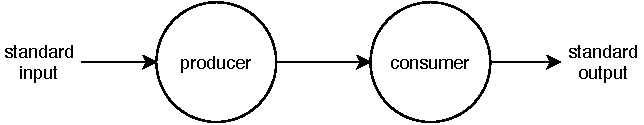
\includegraphics[width=.4 \linewidth]{img/concurrent-c.pdf}

    \begin{lstlisting}
process spec consumer() { trans void send(int); };
process spec producer(process consumer);
process body producer(process consumer cons) {
    int c; while ((c = getchar()) != EOF) cons.send(c);
    cons.send(EOF);
}
process body consumer() {
    int ch; while (1) {
        accept send(c) ch = c;
        if (ch == EOF) break;
        if (islower(ch)) ch = toupper(ch);
        putchar(ch);
    }
}
int main(void) {
    create producer(create consumer()); return 0;
}
    \end{lstlisting}
\end{frame}


\section{FT~Concurrent~C}
\begin{frame}{FT~Concurrent~C}
    \begin{itemize}\setlength\itemsep{2.5em}
        \item
            A~\emph{superset} of \alert{Concurrent~C}. Its extensions include
            facilities for creating \emph{replicated processes}, detection
            of \emph{failure of processes}, automatic termination of
            \emph{slave orphan processes}, etc.

        \item
            \textbf{Assumptions:}

            \begin{enumerate}\setlength\itemsep{1em}
                \item
                    \emph{Processor failure} can be detected.

                \item
                    The processors are \emph{homogeneous} and \emph{fail
                    by stopping}.

                \item
                    Each message is either \emph{transmitted correctly} or
                    \emph{not at all}.

                \item
                    All working processors can communicate with each other.
            \end{enumerate}
    \end{itemize}
\end{frame}


\section{FT~Concurrent~C - Replication Model}
\begin{frame}{FT~Concurrent~C\,--\,Replication Model}
    \begin{itemize}\setlength\itemsep{1em}
        \item
            \emph{Replicated process} behaves like a~\alert{single process}.
            Interaction with a~replicated process \emph{automatically implies
            interaction} with all of its replica processes. All replicas
            generate replies.

        \item
            \alert{First-response approach}\,--\,just the \emph{response of
            the first replica} is taken and the responses of the other
            replicas are \emph{discarded}.

            \begin{itemize}\setlength\itemsep{.3em}
                \item
                    Protects against \emph{processor failures}.

                \item
                    Only \emph{one active replica} is needed for full
                    functionality.

                \item
                    It is \emph{fast} because a~process interacting with
                    a~replicated process does not have to \emph{wait for all
                    the replicas to respond}.

                \item
                    Replicas can \emph{fall behind in execution}.% There is
                    % a~mechanism to ensure the \emph{correct order of external
                    % events}.
            \end{itemize}

        \item
            \textbf{Programmers responsibilities:}

            \begin{enumerate}\setlength\itemsep{.5em}
                \item
                    Decide which processes \emph{should be replicated}.

                \item
                    Ensure that all replicas of a~replicated process have
                    the \emph{same external behaviour}.
            \end{enumerate}
    \end{itemize}
\end{frame}


\section{FT~Concurrent~C - Replicated Processes}
\begin{frame}{FT~Concurrent~C\,--\,Replicated Processes}
    \alert{Creating a~replicated process} with~$ n $~copies, each with
    \emph{identical arguments}:

    \begin{center}
        \texttt{create [slave] process\_type(arguments)} \\
        \texttt{[copies($ \mathrm{n} $) |
        processor($ \mathrm{n_1} $, $ \mathrm{n_2} $, \ldots)]}
    \end{center}

    % An alternative form which allows each replica to be given
    % \emph{different arguments}:

    % \begin{center}
    %     \texttt{create [slave] (process\_type(arguments)
    %     [processor($ \mathrm{n_1} $)],} \\
    %     \texttt{process\_type(arguments) [processor($ \mathrm{n_2} $)], \ldots)}
    % \end{center}

    % \noindent\rule{\linewidth}{.3pt}
    \vspace{1em}

    \begin{itemize}\setlength\itemsep{2em}
        \item
            The operation returns a~\emph{single process identifier}
            which identifies the entire \emph{set of replicas}.

        \item
            The created process can be marked as a~\alert{slave} of the
            parent process. If the parent process \emph{terminates abnormally},
            then all of its slave processes will be \emph{killed}.
    \end{itemize}
\end{frame}


% \section{FT~Concurrent~C - No-Fault Call Operator, Death Notices}
% \begin{frame}{FT~Concurrent~C\,--\,No-Fault Call Operator, Death Notices}
%     \begin{itemize}\setlength\itemsep{2em}
%         \item
%             \textbf{No-Fault Call Operator:}

%             The transaction call syntax is extended by the \alert{no-fault
%             transaction call operator}:

%             \begin{center}
%                 \texttt{transaction\_call\ ??\ fault\_expr}
%             \end{center}

%             If the called process \emph{accepts this call} and \emph{returns
%             a~value}, then that value becomes the value of the expression.
%             Otherwise, \texttt{fault\_expr} is evaluated and its value is used.

%         \item
%             \textbf{Death Notices:}

%             \begin{itemize}\setlength\itemsep{.5em}
%                 \item
%                     The \alert{death notice} mechanism allows a~process to
%                     request a~specific transaction call to be generated when
%                     a~\emph{given process terminates}. There is the built-in
%                     function \texttt{c\_request\_death\_notice} to request
%                     this behaviour.

%                 \item
%                     There is also the built-in function
%                     \texttt{c\_cancel\_death\_notice} for \emph{withdrawal} of
%                     a~death notice request.
%             \end{itemize}
%     \end{itemize}
% \end{frame}


\section{Summary}
\begin{frame}{Summary}
    \begin{itemize}\setlength\itemsep{2em}
        \item
            \alert{FT~Concurrent~C} is a~tool for writing \emph{fault tolerant
            distributed programs}.

        \item
            \emph{Critical program components} (processes) can be made fault
            tolerant by \alert{replicating} them.

        \item
            Interaction with the replicated processes is managed by the
            \alert{run-time system}.

        \item
            The replication is \alert{not for free}. A~price has to be paid because of the:

            \begin{enumerate}\setlength\itemsep{.5em}
                \item
                    extra \emph{transaction calls},

                \item
                    \emph{synchronisation} between replicas,

                \item
                    \emph{programming effort}.
            \end{enumerate}
    \end{itemize}
\end{frame}


\end{document}
